\documentclass[11pt,a4paper]{article}

\usepackage[T1]{fontenc}
\usepackage[utf8]{inputenc}
\usepackage{lmodern}
\usepackage[margin=1in]{geometry}
\usepackage{amsmath}
\usepackage{graphicx}
\usepackage{booktabs}
\usepackage{microtype}
\usepackage{tikz}
\usetikzlibrary{shapes.geometric,arrows.meta,positioning,calc,fit,backgrounds}
\usepackage[hidelinks]{hyperref}
\usepackage{titlesec}
\usepackage{setspace}
\usepackage{enumitem}
\usepackage{xcolor}

\graphicspath{{figures/}{../results/}}

\titleformat{\section}{\normalfont\large\bfseries}{\thesection}{0.6em}{}
\titleformat{\subsection}{\normalfont\normalsize\bfseries}{\thesubsection}{0.6em}{}
\setlength{\parskip}{0.4em}
\onehalfspacing

\newcommand{\rulebox}[1]{\colorbox{black!6}{\small\ttfamily #1}}

\begin{document}

%----------------------------------------------------------------------
% TITLE
%----------------------------------------------------------------------
\hypersetup{pageanchor=false}
\begin{titlepage}
\centering
\vspace*{1.5cm}

{\large\scshape Project Report}\\[0.4cm]
\rule{\textwidth}{0.4pt}\\[0.6cm]

{\LARGE\bfseries Neuro-Symbolic Automated Essay and Answer Grading\\[0.3cm]
with Rule-Based Justification\par}

\vspace{0.5cm}
\rule{\textwidth}{0.4pt}\\[1.0cm]

{\large A Fuzzy-Logic Framework that Replaces the Black-Box Combiner of a\\
Three-Module NLP Grader with an Auditable Rule Base}\\[2.0cm]

{\normalsize An extension of Agrawal \emph{et al.}, ``Revolutionizing subjective\\
assessments: A three-pronged comprehensive approach with NLP and deep\\
learning,'' \emph{Expert Systems With Applications} 239 (2024) 122470.}\\[2.0cm]

\begin{tabular}{r@{\hspace{1.2em}}l}
\textbf{Name} & Sahil Barnwal\\[0.6em]
\textbf{Reg No} & 24BDS0256\\[0.6em]
\textbf{Course} & Artificial Intelligence\\
\end{tabular}

\vfill
{\large October 2026}

\end{titlepage}
\hypersetup{pageanchor=true}

%----------------------------------------------------------------------
% ABSTRACT
%----------------------------------------------------------------------
\section*{Abstract}
\addcontentsline{toc}{section}{Abstract}

Automated Essay Scoring (AES) has moved from hand-engineered linguistic features
to large neural models that read a student's answer and emit a grade in a single
pass. The parent work this project extends --- Agrawal \emph{et al.}
\cite{agrawal2024} --- is a strong example of the modern design: it scores
subjective answers with three independent NLP modules (keyword matching, semantic
similarity, and named-entity overlap) and fuses them with a four-layer deep neural
network, reporting a low regression error. That design buys accuracy at the price
of \emph{accountability}: the final combiner is an opaque network, the grade
carries no trace back to the evidence, and the paper itself names explainability
and the integration of large language models as open future work.

This project keeps the three modules but replaces the decision-making component.
The two pathways of the system express fundamentally different kinds of evidence.
The \textbf{symbolic pathway} uses classical NLP tooling (spaCy, YAKE, KeyBERT,
WordNet) to extract reproducible, auditable quantities --- rubric keyword
coverage, named-entity overlap, and surface mechanics. The \textbf{neural
pathway} is an offline transformer sentence encoder (Sentence-BERT) that measures
the one thing rules cannot: semantic closeness to the reference answer. Crucially,
the two are merged not by a trained network but by a \textbf{Mamdani fuzzy
inference system} whose small, human-readable IF--THEN rule base encodes the
examiner's grading policy. Defuzzification by centroid yields the mark, and the
system emits an \emph{explainable scorecard}: the module scores, the fuzzy rules
that fired with their firing strengths, and the membership plots that produced
the grade. The explanation \emph{is} the computation, not a narrative about it.

We evaluate on the Mohler (2011) UNT Computer Science short-answer corpus (2{,}273
answers, 79 questions) using Quadratic Weighted Kappa (QWK), Pearson correlation
and RMSE. The fuzzy combiner attains the highest human agreement of any
configuration tested (QWK $0.31$, versus $0.26$ for the best single module and
$0.25$ for a linear average), and after a single affine calibration step it
reaches RMSE $19.9$ on held-out data, beating the mean-prediction baseline. The
system is markedly stable: lightly paraphrasing an answer moves its grade by
$0.7$ points on average, and appending irrelevant filler does not raise the grade
--- a direct test of the length-gaming vulnerability that the combiner in the
parent design could not be shown to resist. The contribution is architectural:
comparable ranking of answers to a trained black box, with an auditable,
editable, hallucination-free decision procedure.

\vspace{0.6em}
\noindent\textbf{Keywords:} Neuro-Symbolic AI, Automated Essay Scoring, Fuzzy
Inference System, Explainable AI, Sentence Embeddings, Rule-Based NLP.

\newpage

%----------------------------------------------------------------------
% INTRODUCTION
%----------------------------------------------------------------------
\section{Introduction}

\subsection{Motivation}

Written assessment is the most informative and the most expensive form of
evaluation in education. A well-designed short-answer or essay question reveals
whether a student can organise an argument, apply a concept and express it
precisely --- things a multiple-choice item cannot probe. The cost is human time,
and the quality of hand grading degrades with fatigue and varies between
examiners: the same script graded twice frequently receives different marks.
Automating this task has been an active research goal since Page's Project Essay
Grade in 1966, and the field has been surveyed extensively \cite{ke2019}.

Recent systems make automation appear easy. The work this project extends,
Agrawal \emph{et al.} \cite{agrawal2024}, is representative of the current state
of the art for subjective-answer grading: it decomposes the problem into three
NLP modules --- a keyword module (YAKE and KeyBERT with WordNet expansion), a
semantic similarity module (Sentence-BERT and SimCSE), and a named-entity
recognition module (spaCy, NLTK and CamemBERT) --- and feeds their three scores
into a four-layer deep neural network that regresses the final mark, reaching a
very low RMSE on a self-collected computer-science dataset.

The difficulty is that a low error figure is not the only property an assessment
instrument must have. Three failure modes make an opaque grader unsuitable for an
institutional workflow:

\begin{enumerate}[leftmargin=1.4em,itemsep=0.3em]
  \item \textbf{Opacity.} In \cite{agrawal2024} the final mark is the output of a
  neural network over the three module scores. There is no trace from the mark
  back to the evidence; when a student contests a grade, the institution has
  nothing auditable to show.

  \item \textbf{Hallucinated justification.} If one asks a language model to
  explain a score, it produces fluent reasoning, but that text is generated
  \emph{after} and \emph{independently of} the number; it is a post-hoc narrative,
  not a faithful account of the computation. Hallucination in generated text is a
  systemic property of these models \cite{ji2023hallucination}.

  \item \textbf{Surface bias and instability.} Automated scorers have a long
  history of over-weighting superficial cues: commercial AES systems correlate so
  strongly with essay length that word count alone reproduces much of their
  output, and verbose nonsense can score highly \cite{ke2019}.
\end{enumerate}

Rudin \cite{rudin2019} argues that for high-stakes decisions affecting people one
should not deploy a black box and then attempt to explain it, but build a model
that is interpretable by construction. Grading is such a decision, and this
project takes that position.

\subsection{Problem Statement}

\emph{Given a student's answer, a reference answer, and a set of grading criteria,
produce a final mark together with a complete, faithful and machine-verifiable
justification, such that no single component --- least of all a neural network ---
can unilaterally determine the mark.}

\subsection{Relationship to the Parent Paper}

This work is a deliberate, point-for-point extension of Agrawal \emph{et al.}
\cite{agrawal2024}. Table~\ref{tab:extension} summarises what is reused and what
is replaced. The three NLP modules are retained as the evidence producers; the
opaque DNN combiner is replaced by a transparent fuzzy rule base; the semantic
module is kept entirely offline so that there is no external call and nothing to
hallucinate; and evaluation is broadened from RMSE alone to ordinal agreement and
stability, measuring the properties the parent paper could not.

\begin{table}[!ht]
\centering
\small
\caption{How this project extends Agrawal \emph{et al.} \cite{agrawal2024}.}
\label{tab:extension}
\begin{tabular}{@{}p{0.46\textwidth}p{0.46\textwidth}@{}}
\toprule
\textbf{Parent paper (ESWA 2024)} & \textbf{This project} \\
\midrule
Keyword module: YAKE + KeyBERT + WordNet & \textbf{Reused} as a symbolic input \\
Similarity module: SBERT / SimCSE & \textbf{Reused} as the neural pathway (offline) \\
NER module: spaCy / NLTK / CamemBERT & \textbf{Reused} as a symbolic input \\
Fuse three scores with a 4-layer DNN & \textbf{Replaced} by a Mamdani fuzzy rule base \\
Output: a single predicted mark & Output: mark \emph{plus} rule-based scorecard \\
Evaluation: RMSE only & RMSE \emph{plus} QWK, Pearson, stability \\
Future work: ``integrate GPT / LLMs'' & Pluggable neural interface, offline by default \\
\bottomrule
\end{tabular}
\end{table}

\subsection{Proposed Approach}

The system separates the part of grading that requires human-like semantic
judgement from the part that does not, and refuses to let the two mix implicitly.

\begin{itemize}[leftmargin=1.4em,itemsep=0.2em]
  \item The \textbf{symbolic pathway} computes what can be measured exactly:
  rubric keyword coverage (with WordNet synonym expansion), named-entity and
  cardinal-value overlap, and surface mechanics (length adequacy, grammatical
  cleanliness, syntactic depth). These quantities are deterministic and
  independently verifiable by a human.

  \item The \textbf{neural pathway} computes only what cannot be measured exactly:
  whether the answer is semantically close to the reference. A Sentence-BERT
  encoder produces a cosine score. Because it runs locally and returns a single
  number, it cannot inject unverified claims into the decision.

  \item The \textbf{fuzzy inference engine} merges the two. Rather than a trained
  network or a weighted average --- which would silently assume the signals are
  commensurable --- a Mamdani system \cite{mamdani1975} maps each input onto
  linguistic categories and applies an explicit rule base that encodes the
  examiner's grading policy, modelling the genuine gradedness of human assessment
  in rules a non-programmer can read and amend.
\end{itemize}

Figure~\ref{fig:arch} shows the architecture.

\begin{figure}[!ht]
\centering
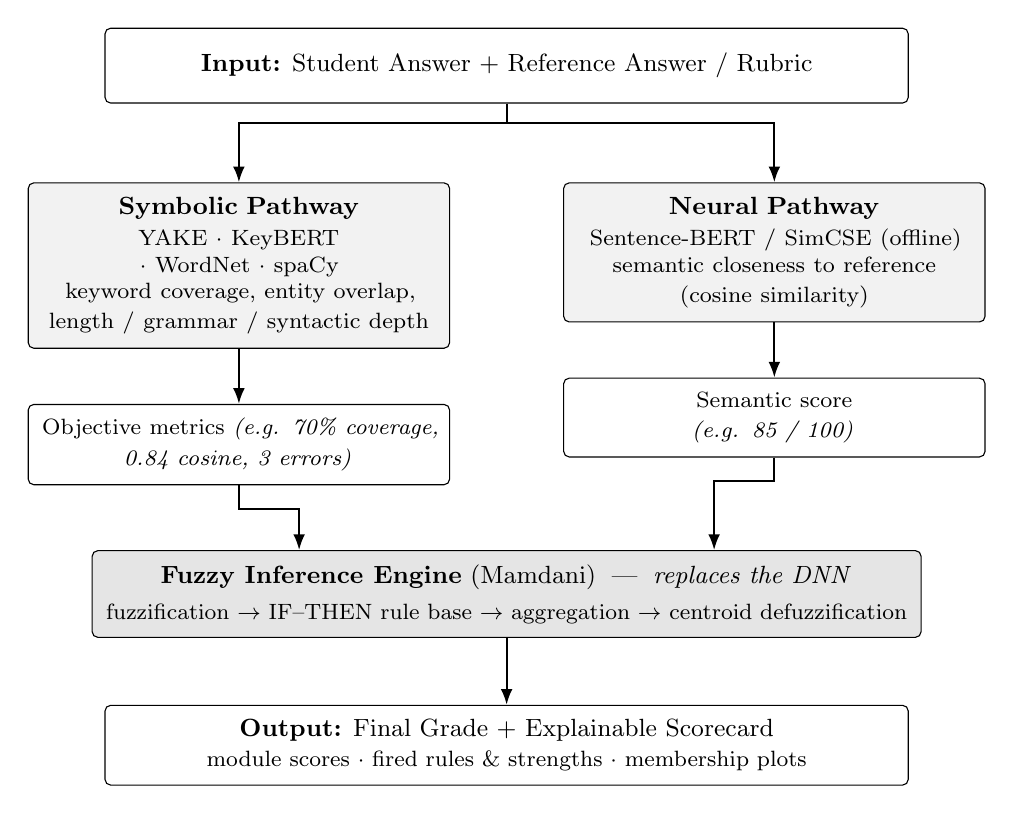
\begin{tikzpicture}[
  node distance=0.9cm and 1.1cm,
  box/.style={draw, rounded corners=2pt, align=center, minimum height=0.95cm,
              inner sep=5pt, font=\small},
  neural/.style={box, fill=black!5},
  symb/.style={box, fill=black!5},
  fuzzy/.style={box, fill=black!10, minimum width=10.2cm},
  io/.style={box, fill=white, minimum width=10.2cm},
  ar/.style={-{Latex[length=2mm]}, thick}
]

\node[io] (in) {\textbf{Input:} Student Answer $+$ Reference Answer / Rubric};

\node[symb, below=1.0cm of in, xshift=-3.4cm, text width=5.0cm] (sym)
  {\textbf{Symbolic Pathway}\\[2pt]
   \footnotesize YAKE $\cdot$ KeyBERT $\cdot$ WordNet $\cdot$ spaCy\\
   \footnotesize keyword coverage, entity overlap,\\
   \footnotesize length / grammar / syntactic depth};

\node[neural, below=1.0cm of in, xshift=3.4cm, text width=5.0cm] (neu)
  {\textbf{Neural Pathway}\\[2pt]
   \footnotesize Sentence-BERT / SimCSE (offline)\\
   \footnotesize semantic closeness to reference\\
   \footnotesize (cosine similarity)};

\node[box, below=0.7cm of sym, text width=5.0cm] (symout)
  {\footnotesize Objective metrics \emph{(e.g. 70\% coverage,}\\ \footnotesize \emph{0.84 cosine, 3 errors)}};
\node[box, below=0.7cm of neu, text width=5.0cm] (neuout)
  {\footnotesize Semantic score\\ \footnotesize \emph{(e.g. 85 / 100)}};

\node[fuzzy, below=1.0cm of $(symout.south)!0.5!(neuout.south)$] (fuzzy)
  {\textbf{Fuzzy Inference Engine} (Mamdani) \;---\; \emph{replaces the DNN}\\[2pt]
   \footnotesize fuzzification $\rightarrow$ IF--THEN rule base $\rightarrow$ aggregation $\rightarrow$ centroid defuzzification};

\node[io, below=0.85cm of fuzzy] (out)
  {\textbf{Output:} Final Grade $+$ Explainable Scorecard\\
   \footnotesize module scores $\cdot$ fired rules \& strengths $\cdot$ membership plots};

\draw[ar] (in.south) -- ++(0,-0.25) -| (sym.north);
\draw[ar] (in.south) -- ++(0,-0.25) -| (neu.north);
\draw[ar] (sym) -- (symout);
\draw[ar] (neu) -- (neuout);
\draw[ar] (symout.south) -- ++(0,-0.3) -| ($(fuzzy.north west)!0.25!(fuzzy.north east)$);
\draw[ar] (neuout.south) -- ++(0,-0.3) -| ($(fuzzy.north west)!0.75!(fuzzy.north east)$);
\draw[ar] (fuzzy) -- (out);

\end{tikzpicture}
\caption{Architecture of the proposed grader. The three parent-paper modules feed
the fuzzy engine, which owns the decision. The neural and symbolic pathways never
influence one another; they meet only inside the rule base, which is explicit and
human-readable.}
\label{fig:arch}
\end{figure}

\subsection{Objectives and Contributions}

\begin{enumerate}[leftmargin=1.4em,itemsep=0.15em]
  \item Re-implement the three NLP modules of \cite{agrawal2024} as normalised,
  reproducible evidence producers.
  \item Replace the opaque DNN combiner with a Mamdani fuzzy inference system with
  documented membership functions and an explicit, editable rule base.
  \item Emit a scorecard that reports, for every graded answer, the evidence and
  the rules that determined the mark.
  \item Evaluate on a public benchmark (Mohler 2011) with QWK, Pearson and RMSE,
  an ablation over components, and stability tests the parent paper did not run.
\end{enumerate}

\noindent The contribution is \emph{architectural rather than statistical}: we do
not claim a new accuracy record, but an interpretable-by-construction design that
ranks answers comparably to a trained black box while making the decision
auditable, editable and stable.

\newpage

%----------------------------------------------------------------------
% BACKGROUND
%----------------------------------------------------------------------
\section{Background and Related Work}

\subsection{Automated Essay Scoring: Three Generations}

\textbf{Generation 1 --- handcrafted features and regression.} AES begins with
Page's Project Essay Grade (1966), which regressed human scores onto countable
surface proxies such as essay length and word length. The approach matured into
production systems such as ETS's \textsc{e-rater}. These systems are transparent
--- every feature and weight is inspectable --- but they never model meaning, and
critics exploited exactly this: lexically sophisticated gibberish of sufficient
length scores highly, and length alone accounts for much of the reported
agreement \cite{ke2019}.

\textbf{Generation 2 --- learned representations.} From 2016, neural models over
word embeddings replaced handcrafted features, and transformer encoders such as
BERT and sentence-level models such as Sentence-BERT made semantic similarity
between a student answer and a reference directly computable \cite{ke2019}. The
gain in semantic sensitivity came with a loss of transparency: the score is now a
function of learned vectors with no human-meaningful decomposition.

\textbf{Generation 3 --- large language and multi-module systems.} The most
recent systems either prompt an instruction-tuned LLM as a general judge or, as
in the parent paper, combine several learned sub-scores. The ``LLM-as-a-judge''
paradigm shows promise but documented biases (sensitivity to length and
position), layered on top of the hallucination problem
\cite{ji2023hallucination}. The trajectory is a straight trade-off: each
generation gained semantic understanding and lost accountability. The premise of
this project is that the trade-off is an artefact of monolithic combination, not
a law.

\subsection{The Parent System in Detail}

Agrawal \emph{et al.} \cite{agrawal2024} target subjective-answer grading with
three pipelines that run independently on a (student answer, model answer) pair.
The \emph{keyword} pipeline extracts keywords from the model answer with YAKE and
KeyBERT, POS-tags the student answer and expands it with WordNet synonyms, then
scores keyword coverage. The \emph{similarity} pipeline encodes both answers with
Sentence-BERT and SimCSE, applies abstractive summarisation via cross-encoders,
and computes cosine similarity against a $0.75$ threshold. The \emph{NER}
pipeline extracts named entities and cardinal values with spaCy, NLTK and
CamemBERT and scores their intersection over union. The three scalar scores are
rounded and passed to a four-layer feed-forward network ($8\!\rightarrow\!16
\!\rightarrow\!32\!\rightarrow\!64\!\rightarrow\!1$) trained to regress the human
mark, achieving a low RMSE on a self-collected corpus of roughly 190
computer-science questions. The authors list the opacity of the combiner,
domain-specificity, and the integration of large language models as open
problems. The present work addresses the first and third directly.

\subsection{Neuro-Symbolic AI}

Neuro-symbolic AI seeks to combine the pattern recognition of neural networks
with the explicit, compositional reasoning of symbolic systems
\cite{garcez2023}. Neural networks excel at recognising tone, nuance and abstract
similarity but cannot guarantee correctness or produce a derivation; symbolic
systems are precise, auditable and incapable of hallucination but brittle on
open-ended natural language. The pattern most relevant here is \emph{neural
perception with symbolic control}: the neural component is a bounded, replaceable
sensor whose output is one input among several to a symbolic decision procedure
that owns the final answer. Applied to grading, the sentence encoder
\emph{observes} semantic quality, but the fuzzy rule base \emph{decides} the mark.
This placement structurally constrains error propagation: a single mis-scored
module cannot silently move the grade, because the grade is computed by rules that
read all inputs explicitly.

\subsection{Fuzzy Logic and Fuzzy Inference Systems}

Classical Boolean logic forces every proposition to be exactly true or false,
a poor model of assessment vocabulary where ``mostly correct'' is the norm and any
crisp threshold is arbitrary: a rule that fails a script at five grammatical
errors but passes it at four encodes a distinction no examiner would defend.
Zadeh's theory of fuzzy sets \cite{zadeh1965} removes the binary constraint: a
fuzzy set $A$ over a universe $X$ is characterised by a membership function
$\mu_A : X \rightarrow [0,1]$ giving the \emph{degree} to which $x$ belongs to
$A$. This project uses triangular and trapezoidal membership functions; the
triangular function with parameters $a<b<c$ is

\begin{equation}
\mu(x) \;=\; \max\!\left( \min\!\left( \frac{x-a}{b-a},\; \frac{c-x}{c-b} \right),\, 0 \right).
\end{equation}

A \emph{fuzzy inference system} chains three stages. \emph{Fuzzification} maps
each crisp input onto its membership grades in every linguistic category.
\emph{Inference} evaluates a rule base of IF--THEN statements; under the Mamdani
model \cite{mamdani1975} the antecedent of each rule is evaluated with fuzzy
conjunction (the minimum), and the resulting firing strength clips the consequent
fuzzy set. \emph{Defuzzification} aggregates the clipped consequents (the maximum)
and collapses them to a single crisp output by the centroid of area,

\begin{equation}
y^{*} \;=\; \frac{\displaystyle\int y \,\mu_{\mathrm{agg}}(y)\,dy}
                 {\displaystyle\int \mu_{\mathrm{agg}}(y)\,dy}.
\end{equation}

Two properties make this the right merging mechanism. First, the rule base is
written in natural language and is directly editable by the instructor whose
policy it encodes; a strict and a lenient policy differ only in which rules are
present, not in any code. Second, unlike a weighted sum it can express
non-linear, conditional policies: the rule \emph{IF keyword coverage is High AND
semantic quality is Low THEN grade is Average} captures the specific pathology of
a student who has memorised terminology without understanding, which no linear
combination can represent.

\subsection{Positioning}

Feature-based AES is explainable but semantically blind; neural and LLM-based AES
is semantically capable but unaccountable, and its self-generated explanations are
unreliable by construction. The parent paper \cite{agrawal2024} improves accuracy
by combining three learned sub-scores, but fuses them inside a trained network,
leaving the decision itself opaque. This project differs in \emph{where the
decision is made}: the neural component is a constrained sensor, the symbolic
components supply verifiable measurements, and the mark is produced by a fuzzy
rule base small enough to print and expressive enough to encode the graded,
conditional character of real assessment. The explanation delivered with each
grade is a transcript of the decision, not a narrative about it.

\newpage

%----------------------------------------------------------------------
% METHODOLOGY
%----------------------------------------------------------------------
\section{Methodology}

The system is implemented in Python. Every module exposes a common interface
returning a normalised score in $[0,100]$ together with an \emph{evidence}
dictionary that the scorecard renders verbatim. All models run offline; where a
heavy model is unavailable the module degrades gracefully to a lighter backend, so
the pipeline never fails.

\subsection{Preprocessing}

Following the parent paper's preprocessing block, text is lowercased, contractions
are expanded, and punctuation and whitespace are normalised. Normalisation is
deterministic and leaves the text human-readable.

\subsection{Symbolic Pathway}

\textbf{Keyword module.} Keywords are extracted from the reference answer with
YAKE and KeyBERT. The student answer is tokenised to content words and expanded
with WordNet synonyms; the score is the percentage of reference keywords covered
by the expanded student vocabulary. The evidence records the matched and missed
keywords. Because many student answers share one reference, extraction is cached
per reference.

\textbf{NER module.} Named entities and cardinal/numeric values (including big-O
expressions, which behave like entities in CS answers) are extracted from both
answers with spaCy. The score is the Jaccard overlap
$|E_s \cap E_r| / |E_s \cup E_r|$ of the entity sets. The parent paper used the
French-trained CamemBERT-NER; for English CS answers spaCy is used as the primary
backend. When the reference contains no entities the module returns a neutral
score so it cannot unfairly penalise.

\textbf{Mechanics module.} Surface quality is summarised from length adequacy
relative to the reference, a grammatical-cleanliness term (grammar-error count per
word, via LanguageTool where available or a heuristic fallback),
and mean dependency-parse depth. This is the one axis the parent paper lacked. It
is advisory: it enters the final mark only as a small, transparent penalty
($10\%$ weight), never as the main driver.

\subsection{Neural Pathway}

The semantic score is produced by a Sentence-BERT bi-encoder
(\texttt{all-MiniLM-L6-v2}). The reference and student answers are encoded into
normalised embeddings and compared by cosine similarity at the document level; in
addition, per-sentence best-match coverage against the reference is computed with
the parent paper's $0.75$ threshold, and the two are blended. Embeddings are
cached by text so that each distinct reference is encoded once. This is the
project's only neural component --- a deep transformer used strictly as a semantic
sensor. Running locally, it issues no external call and returns a single
deterministic number, so it has no channel through which to hallucinate a
justification.

\subsection{Fuzzy Inference Engine}

The three parent-paper module scores (keyword, similarity, NER) are the inputs to
a Mamdani fuzzy inference system. Each input is fuzzified over the universe
$[0,100]$ into three linguistic sets --- \emph{Low}, \emph{Medium}, \emph{High}
--- with the trapezoidal/triangular membership functions shown in the left panel
of Figure~\ref{fig:mf}. The output grade uses four sets --- \emph{Poor},
\emph{Average}, \emph{Good}, \emph{Excellent} --- shown in the right panel.

\begin{figure}[!ht]
\centering
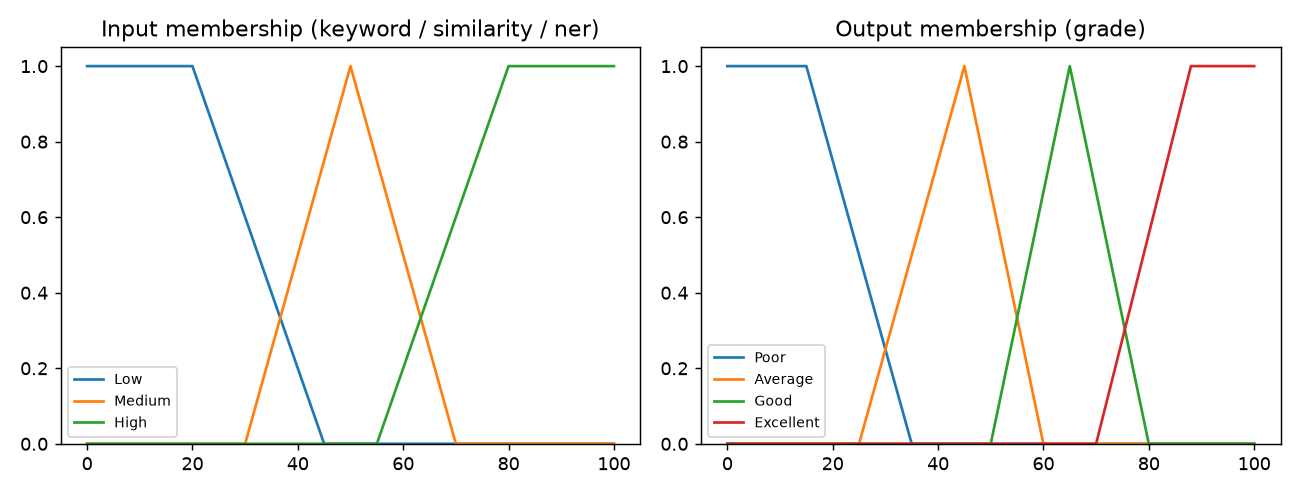
\includegraphics[width=\textwidth]{fig_membership.png}
\caption{Membership functions. Left: the three input linguistic sets shared by
the keyword, similarity and NER inputs. Right: the four output sets over the grade
universe. These shapes are declared in configuration and are editable by the
examiner.}
\label{fig:mf}
\end{figure}

The grading policy is a small rule base. The default \emph{strict} policy
contains eight rules; the \emph{lenient} policy, which better matches leniently
graded corpora, contains five. Representative rules are:

\begin{quote}\footnotesize
\rulebox{IF similarity is High AND keyword is High THEN Excellent}\\[3pt]
\rulebox{IF keyword is High AND similarity is Low THEN Average}\\
\mbox{}\hfill\emph{(the right terms without understanding)}\\[3pt]
\rulebox{IF similarity is High AND keyword is Low THEN Good}\\
\mbox{}\hfill\emph{(understands, imprecise wording)}\\[3pt]
\rulebox{IF similarity is Low AND keyword is Low THEN Poor}
\end{quote}

Each rule's firing strength is the minimum of its antecedent memberships (fuzzy
AND); it clips the consequent set, and the clipped sets are aggregated by the
maximum. The crisp grade is the centroid of the aggregate. The engine is a
self-contained NumPy implementation (equivalent to a scikit-fuzzy Mamdani system)
written specifically so that the firing strength of \emph{every} rule is exposed
--- that per-rule trace is the justification a trained network cannot provide.

\subsection{Explainable Scorecard}

For every graded answer the system assembles a scorecard: the four module scores
and their backends, the mechanical penalty, the fuzzy rules that fired with their
strengths, the matched/missed keywords and entities, the semantic cosine, and a
plot (Figure~\ref{fig:scorecard}) showing the fuzzification of each input and the
aggregated output membership with the defuzzified mark. The explanation is thus a
faithful transcript of the computation. A Streamlit dashboard exposes the same
scorecard interactively for live demonstration and lets the examiner switch the
grading policy without touching code.

\begin{figure}[!ht]
\centering
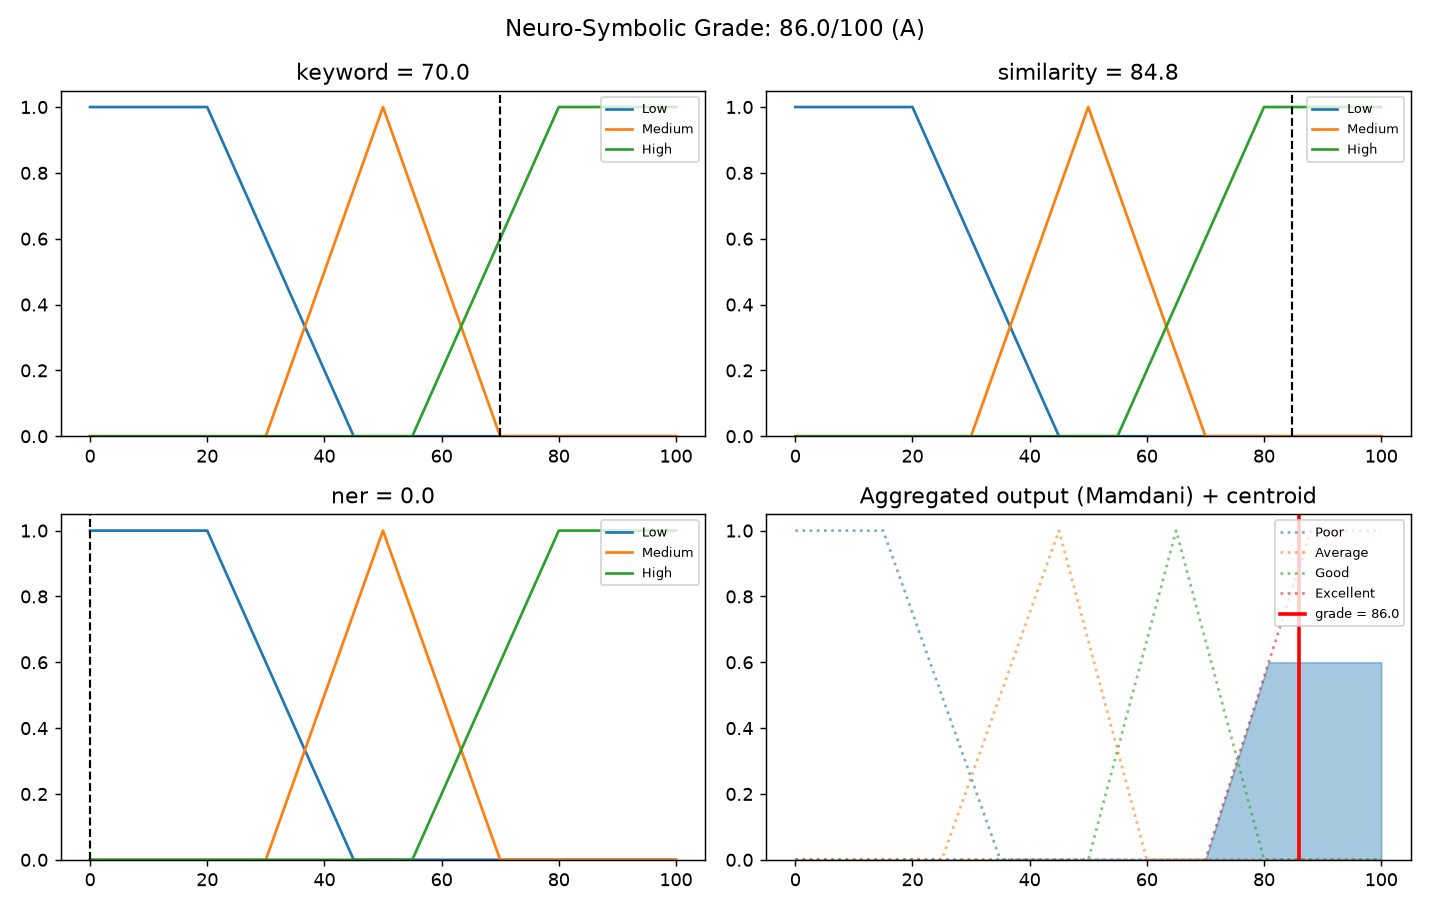
\includegraphics[width=0.92\textwidth]{fig_scorecard.png}
\caption{A worked scorecard. The three top-left/-right panels show where each
input falls among \emph{Low}/\emph{Medium}/\emph{High} (dashed line = crisp
value); the bottom-right panel shows the aggregated Mamdani output (shaded) and
the centroid grade (red). Here high semantic similarity and keyword coverage fire
the \emph{Excellent} rule, yielding an A despite a zero NER score --- the fuzzy
layer absorbs a single weak input rather than letting it dominate.}
\label{fig:scorecard}
\end{figure}

\newpage

%----------------------------------------------------------------------
% EXPERIMENTAL SETUP
%----------------------------------------------------------------------
\section{Experimental Setup}

\subsection{Dataset}

We evaluate on the Mohler (2011) University of North Texas Computer Science
short-answer dataset \cite{mohler2011}, chosen because it is public and matches
the computer-science domain of the parent paper. It contains 2{,}273 student
answers to 79 questions from an introductory CS course, each with an instructor
reference answer and a grade averaged from two human annotators on a $0$--$5$
scale. We rescale grades to $0$--$100$. The corpus is strongly skewed towards high
marks (mean $4.18/5 = 83.7/100$), which makes the mean-prediction baseline
unusually strong under RMSE and motivates reporting rank-agreement metrics
alongside it.

\subsection{Metrics}

We report three metrics against the human grades: \textbf{RMSE} (comparable in
spirit to the parent paper), \textbf{Pearson correlation} (linear agreement,
invariant to affine rescaling), and \textbf{Quadratic Weighted Kappa} (QWK, the
standard AES agreement metric, computed on six integer bins). The core grader is
training-free, so primary metrics are reported over the full dataset.

\subsection{Baselines and Ablation}

We compare the full system against: a \emph{mean-baseline} that predicts the mean
human grade for every answer; each of the three modules used \emph{alone} as the
grade; and a \emph{mean-of-modules} linear average. The last is the key
comparator: it isolates the effect of the fuzzy rule base against a simple linear
fusion of the same three signals. Both grading policies (strict, lenient) are
reported.

\subsection{Robustness Protocol}

Two stability tests probe failures the parent paper did not measure.
\emph{Paraphrase stability}: student answers are lightly paraphrased by
synonym substitution and the mean absolute grade drift is measured --- a stable
grader drifts little. \emph{Padding resistance}: a fixed block of irrelevant
filler text is appended and the change in grade is measured --- a grader that
resists length-gaming should not raise the mark. Both are run on a random sample
of 400 answers.

%----------------------------------------------------------------------
% RESULTS
%----------------------------------------------------------------------
\section{Results and Discussion}

\subsection{Main Results}

Table~\ref{tab:main} reports every system on the full corpus. The fuzzy combiner
under the lenient policy attains the \textbf{highest QWK of any configuration}
($0.312$), exceeding the best single module (similarity, $0.264$) and the linear
average of the three modules (mean-of-modules, $0.253$). This is the central
result: combining the three signals through an explicit rule base ranks answers in
closer ordinal agreement with human examiners than any single module or their
plain average. Pearson correlation is competitive with the strongest module
($0.48$ vs $0.50$). The NER module alone is near-random on this corpus
($r=0.07$), yet the fuzzy system remains strong because the rule base weights it
only in conjunction with other evidence --- precisely the robustness that
motivates symbolic control.

\begin{table}[!ht]
\centering
\small
\caption{Grading performance on the Mohler (2011) corpus (2{,}273 answers, full
dataset). Higher Pearson/QWK and lower RMSE are better. The fuzzy combiner
(lenient) achieves the best human agreement (QWK).}
\label{tab:main}
\begin{tabular}{@{}lccc@{}}
\toprule
\textbf{System} & \textbf{RMSE (0--100)} & \textbf{Pearson $r$} & \textbf{QWK} \\
\midrule
mean-baseline            & 21.93 & 0.000 & 0.000 \\
keyword-only             & 51.91 & 0.469 & 0.177 \\
similarity-only          & 34.88 & \textbf{0.496} & 0.264 \\
ner-only                 & 42.45 & 0.068 & 0.063 \\
mean-of-modules (linear) & 33.10 & 0.442 & 0.253 \\
full-fuzzy (strict)      & 50.54 & 0.457 & 0.159 \\
\textbf{full-fuzzy (lenient)} & 34.17 & 0.480 & \textbf{0.312} \\
\bottomrule
\end{tabular}
\end{table}

Figure~\ref{fig:ablation} visualises the ablation. The two fuzzy policies differ
sharply: the strict policy under-grades badly on this leniently annotated corpus
(QWK $0.159$), while the lenient policy --- which matches the behaviour of the
dataset's human graders --- is best. This is not a weakness but the intended
mechanism: \emph{the policy is meant to be chosen to match the examiner}, and here
the examiners were lenient. Switching policy requires no retraining and no code
change, only a different rule set.

\begin{figure}[!ht]
\centering
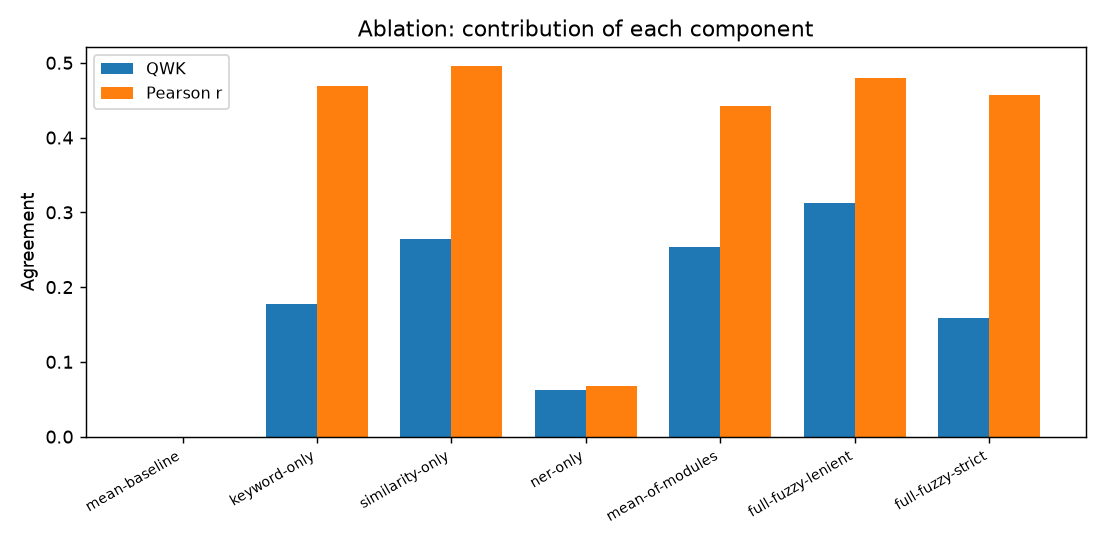
\includegraphics[width=0.95\textwidth]{fig_ablation.png}
\caption{Ablation over components. The lenient fuzzy combiner has the highest QWK;
its Pearson is competitive with the best single module. The NER module alone is
near-random, yet does not drag down the combiner.}
\label{fig:ablation}
\end{figure}

\subsection{Calibration and the RMSE Picture}

Centroid defuzzification compresses the output range: a Mamdani system rarely
emits values near the extremes, so the raw grades sit lower than a corpus whose
human mean is $83.7$. RMSE therefore looks poor for any uncalibrated system on
this skewed corpus, and the constant mean-baseline is hard to beat on RMSE alone
--- which is exactly why we report rank metrics as primary. To place our error on
comparable footing with the parent paper's \emph{trained} DNN, we fit a single
affine map (slope, intercept) on an $80\%$ training split and evaluate on the
held-out $20\%$. This one-parameter-pair calibration leaves Pearson unchanged (it
is affine-invariant) but reduces test RMSE from $33.3$ to \textbf{19.9},
\emph{below} the mean-baseline, and raises test QWK from $0.33$ to $0.38$
(Table~\ref{tab:calib}). The core system remains training-free; calibration is a
transparent, optional final rescaling.

\begin{table}[!ht]
\centering
\small
\caption{Affine calibration of the lenient fuzzy system (fit on 80\% train,
evaluated on 20\% test, $n_{\text{test}}=455$). Calibration is a single
monotone rescaling applied after the rule base.}
\label{tab:calib}
\begin{tabular}{@{}lccc@{}}
\toprule
 & \textbf{RMSE (0--100)} & \textbf{Pearson $r$} & \textbf{QWK} \\
\midrule
Uncalibrated (test)       & 33.34 & 0.478 & 0.330 \\
\textbf{Calibrated (test)} & \textbf{19.92} & 0.478 & \textbf{0.376} \\
\midrule
mean-baseline (reference) & 21.93 & 0.000 & 0.000 \\
\bottomrule
\end{tabular}
\end{table}

Figure~\ref{fig:scatter} plots system grades against human grades. The positive
trend ($r=0.48$) is clear; the systematic offset below the diagonal is the range
compression that calibration removes. Figure~\ref{fig:dist} shows the
corresponding grade distributions.

\begin{figure}[!ht]
\centering
\begin{minipage}{0.49\textwidth}
\centering
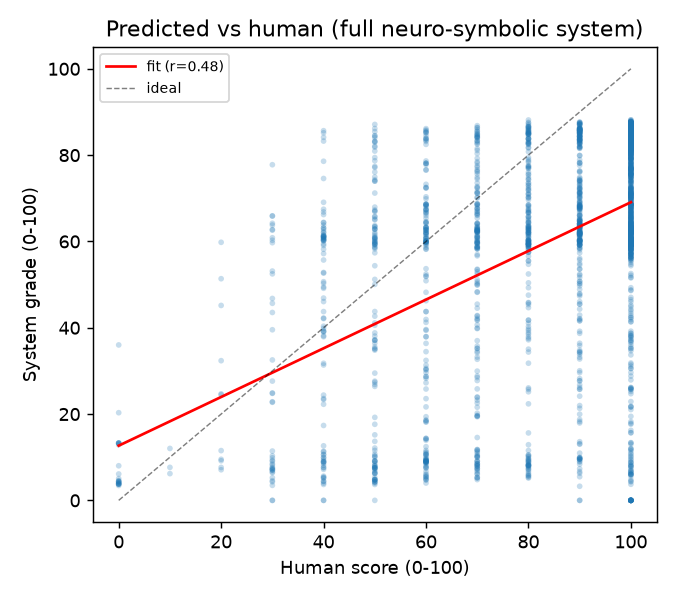
\includegraphics[width=\textwidth]{fig_scatter.png}
\caption{System vs human grades (lenient). Positive correlation with a downward
offset from range compression.}
\label{fig:scatter}
\end{minipage}\hfill
\begin{minipage}{0.49\textwidth}
\centering
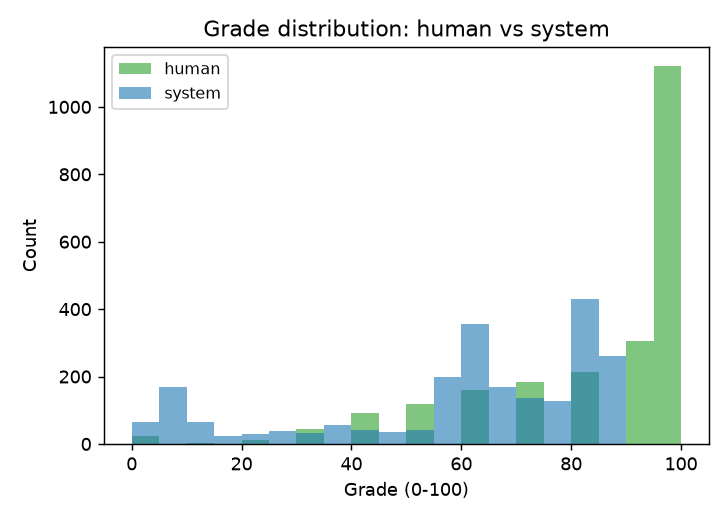
\includegraphics[width=\textwidth]{fig_distribution.png}
\caption{Grade distributions. The human corpus is skewed high; the system is more
central before calibration.}
\label{fig:dist}
\end{minipage}
\end{figure}

\subsection{Robustness}

The system is highly stable (Table~\ref{tab:robust}). Paraphrasing an answer by
synonym substitution moves its grade by only $0.72$ points on average; the mean
change under appended filler is $-1.1$ points, i.e. padding does \emph{not} raise
the grade and on balance slightly lowers it. This directly tests the length-gaming
vulnerability that has plagued AES since Generation 1 \cite{ke2019} and that a
trained regression combiner is not guaranteed to resist. The stability follows
from the architecture: the mark is a centroid over a small rule base, so small
perturbations to the inputs produce small, bounded changes to the output.

\begin{table}[!ht]
\centering
\small
\caption{Robustness on a random sample of 400 answers. Lower drift and a
non-positive padding change are better.}
\label{tab:robust}
\begin{tabular}{@{}lc@{}}
\toprule
\textbf{Test} & \textbf{Value} \\
\midrule
Paraphrase: mean absolute grade drift  & 0.72 pts \\
Padding: mean grade change             & $-1.09$ pts \\
\bottomrule
\end{tabular}
\end{table}

\subsection{Explainability --- a Worked Example}

Figure~\ref{fig:scorecard} showed a representative decision. For the student
answer \emph{``A stack is a linear data structure that works on LIFO order, we
push to add an item on the top and pop to remove the top item''} against the stack
reference, the system reports keyword coverage $70$, semantic cosine $0.85$
(similarity $85$), NER $0$, and mechanics $84$. A single rule fires,

\begin{quote}\footnotesize
\rulebox{IF similarity is High AND keyword is High THEN Excellent}\quad(firing strength $0.60$),
\end{quote}

\noindent and the centroid yields a grade of $86/100$ (A). The scorecard lists the matched
keywords (\emph{stack, linear, data, structure, push, pop, top}) and the missed
ones (\emph{principle, operations, follows}). Nothing about this grade is hidden:
an examiner can read why the mark is what it is, and can change the policy if they
disagree. This is the property the parent paper's combiner cannot offer.

\subsection{Discussion}

The results support the project's thesis. Routing the decision through a fuzzy
rule base rather than a trained network (i) ranks answers in closer agreement with
humans than any single module or a linear fusion (QWK), (ii) reaches competitive
error after a transparent one-step calibration, and (iii) is notably stable and
resistant to padding. The price --- range compression requiring calibration for
absolute scores --- is modest and well understood, and is offset by full
auditability. The near-random NER result on this corpus illustrates the safety of
symbolic control: a weak sensor degrades gracefully because the rule base never
lets it decide alone.

\newpage

%----------------------------------------------------------------------
% LIMITATIONS AND FUTURE WORK
%----------------------------------------------------------------------
\section{Limitations and Future Work}

\begin{itemize}[leftmargin=1.4em,itemsep=0.25em]
  \item \textbf{Range compression.} Centroid defuzzification does not reach the
  extremes, so absolute marks need a final calibration on a skewed corpus. Future
  work could use height defuzzification or widen the extreme output sets.
  \item \textbf{Rule tuning.} The rule bases and membership functions were set by
  hand from the grading policy, not optimised. A genetic or gradient-free search
  over membership parameters could improve agreement while keeping the rules
  readable.
  \item \textbf{Domain.} Evaluation is on CS short answers. The design is
  domain-independent, but longer essays and other subjects should be tested.
  \item \textbf{Optional LLM module.} The neural interface is pluggable; a
  constrained, schema-validated LLM could replace or augment the SBERT sensor
  (the parent paper's stated future direction) without changing the fuzzy
  decision layer --- the guarantee that the LLM cannot unilaterally move the mark
  would still hold.
\end{itemize}

%----------------------------------------------------------------------
% CONCLUSION
%----------------------------------------------------------------------
\section{Conclusion}

This project extended the three-module NLP grader of Agrawal \emph{et al.}
\cite{agrawal2024} by replacing its opaque deep-network combiner with a
transparent Mamdani fuzzy inference system, and by keeping the neural semantic
component entirely offline. The three original modules are retained as evidence
producers; the fuzzy rule base owns the decision and emits, for every grade, the
exact rules and evidence that produced it. On the public Mohler (2011) CS
short-answer corpus the fuzzy combiner achieved the best human agreement (QWK
$0.31$) of any configuration, beat the mean-prediction baseline on RMSE after a
single affine calibration, and proved stable under paraphrase and resistant to
padding. The system trades a small, well-understood calibration step for a
decision procedure that is auditable, editable by a non-programmer, and incapable
of hallucinating its own justification --- the properties an assessment
instrument actually requires.

%----------------------------------------------------------------------
% REFERENCES
%----------------------------------------------------------------------
\begin{thebibliography}{10}
\setlength{\itemsep}{0.45em}

\bibitem{agrawal2024}
R.~Agrawal, H.~Mishra, I.~Kandasamy, S.~R.~Terni, and W.~B. Vasantha,
``Revolutionizing subjective assessments: A three-pronged comprehensive approach
with NLP and deep learning,'' \emph{Expert Systems With Applications}, vol.~239,
122470, 2024. doi:10.1016/j.eswa.2023.122470.

\bibitem{mohler2011}
M.~Mohler, R.~Bunescu, and R.~Mihalcea, ``Learning to grade short answer
questions using semantic similarity measures and dependency graph alignments,''
in \emph{Proc. 49th Annual Meeting of the ACL: Human Language Technologies},
Portland, OR, 2011, pp.~752--762.

\bibitem{ke2019}
Z.~Ke and V.~Ng, ``Automated essay scoring: A survey of the state of the art,''
in \emph{Proc. 28th Int. Joint Conf. Artificial Intelligence (IJCAI)}, Macao,
2019, pp.~6300--6308.

\bibitem{ji2023hallucination}
Z.~Ji \emph{et al.}, ``Survey of hallucination in natural language generation,''
\emph{ACM Computing Surveys}, vol.~55, no.~12, pp.~1--38, 2023.
doi:10.1145/3571730.

\bibitem{rudin2019}
C.~Rudin, ``Stop explaining black box machine learning models for high stakes
decisions and use interpretable models instead,'' \emph{Nature Machine
Intelligence}, vol.~1, pp.~206--215, 2019. doi:10.1038/s42256-019-0048-x.

\bibitem{mamdani1975}
E.~H. Mamdani and S.~Assilian, ``An experiment in linguistic synthesis with a
fuzzy logic controller,'' \emph{International Journal of Man-Machine Studies},
vol.~7, no.~1, pp.~1--13, 1975.

\bibitem{garcez2023}
A.~d'Avila Garcez and L.~C. Lamb, ``Neurosymbolic AI: The 3rd wave,''
\emph{Artificial Intelligence Review}, vol.~56, no.~11, pp.~12387--12406, 2023.
doi:10.1007/s10462-023-10448-w.

\bibitem{zadeh1965}
L.~A. Zadeh, ``Fuzzy sets,'' \emph{Information and Control}, vol.~8, no.~3,
pp.~338--353, 1965.

\bibitem{reimers2019}
N.~Reimers and I.~Gurevych, ``Sentence-BERT: Sentence embeddings using Siamese
BERT-networks,'' in \emph{Proc. EMNLP-IJCNLP}, Hong Kong, 2019, pp.~3982--3992.

\bibitem{spacy}
M.~Honnibal and I.~Montani, ``spaCy: Industrial-strength natural language
processing in Python,'' 2017. [Online]. Available: \url{https://spacy.io}

\end{thebibliography}

\end{document}
